%\documentclass[handout]{beamer} % Sin animaciones
% https://tex.stackexchange.com/questions/74805/latex-error-option-clash-for-package-xcolor
\documentclass[xcolor={dvipsnames},spanish]{beamer}
%\usetheme{Warsaw}
\usetheme{Madrid}
\setbeamertemplate{navigation symbols}{} % remove navigation symbols
%\setbeamercolor{alerted text}{fg=orange}

\usepackage{thesis}
\usepackage{sections/nd_rules}
\setbeamertemplate{footline}[frame number]

\usepackage{cancel} % https://tex.stackexchange.com/questions/23711/strikethrough-text
% https://tex.stackexchange.com/questions/362077/line-jump-using-the-xcancel-macro-in-beamer/362236#362236
\newcommand<>{\xxcancel}[1]{\alt#2{\xcancel{#1}}{\vphantom{\xcancel{#1}}#1}}%uncover the xcancel command

\usepackage{pifont}
\newcommand{\xmark}{\ding{55}}

% https://tex.stackexchange.com/questions/464916/listing-inside-a-frame-using-beamer
\lstset{language=ppa, xleftmargin=0.5cm}

\renewcommand{\lstlistingname}{Programa}

\newcommand{\fForm}{F}
\newcommand{\cForm}{C}

\usepackage{fitch}

% https://tex.stackexchange.com/questions/178800/creating-sections-each-with-title-pages-in-beamers-slides
\AtBeginSection[]{
  \begin{frame}
  \vfill
  \centering
  \begin{beamercolorbox}[sep=8pt,center,shadow=true,rounded=true]{title}
    \usebeamerfont{title}\insertsectionhead\par%
  \end{beamercolorbox}
  \vfill
  \end{frame}
}

\AtBeginSubsection[]{
  \begin{frame}
  \vfill
  \centering
  \begin{beamercolorbox}[sep=8pt,center,shadow=true,rounded=true]{title}
    \usebeamerfont{title}\insertsubsectionhead\par%
  \end{beamercolorbox}
  \vfill
  \end{frame}
}

\newenvironment{command}
    {
        \begin{beamercolorbox}[sep=8pt,center,shadow=true,rounded=true]{block body}
    }
    {\end{beamercolorbox}}


% Justificaciones
\newcommand{\just}[1]{\textcolor{violet}{(#1)}}

% Tiempo total para dar la presentación: 60 minutos, 15 para preguntas
% cada diapo 1-2m. 50 diapos.

% Notas

\title{PPA}
\subtitle{Un asistente de demostración para
lógica de primer orden con extracción de
testigos usando la traducción de Friedman}
\author{Manuel Panichelli}
\institute{
    \textbf{Director}: Pablo Barenbaum

    \textbf{Jurado}: Verónica Becher, Miguel Pagano (FaMAF, UNC)

    Departamento de Computación, FCEyN, UBA
}

\date{Diciembre 2024}

\begin{document}


\frame{\titlepage}

\section{Introducción}

\begin{frame}{Repaso de lógica}
    \begin{definitions}[Conceptos centrales]
        \begin{itemize}
            \item \textbf{Axioma}: Afirmación se declara \textit{siempre válida} (sin demostración).
            \item \textbf{Teorema}: Afirmación que puede ser \textit{demostrada}.
            \item \textbf{Demostración}:
            \begin{itemize}
                \item \textit{Argumento} que establece que un teorema es cierto.
                \item Usa \textit{reglas de inferencia} a partir de \textit{axiomas} y otros teoremas.
                \item Enmarcada en un \textit{sistema deductivo}.
            \end{itemize} 
        \end{itemize}
    \end{definitions}
\end{frame}

\begin{frame}{Ejemplo de teorema}
    \begin{example}[Teorema de Pitágoras]
        \begin{columns}
            \begin{column}{0.5\textwidth}
                \[
                a^2 + b^2 = c^2.
                \]
            \end{column}
            \begin{column}{0.5\textwidth}
                \begin{figure}[H]
                    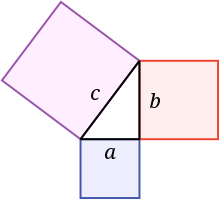
\includegraphics[scale=0.4]{img/ppt/pitagoras.png}
                \end{figure}
            \end{column}
        \end{columns}
        \begin{itemize}
            \item \textbf{Sistema}: Geometría euclidiana.
            \item \textbf{Axioma}: Se puede dibujar una línea recta entre dos puntos.
        \end{itemize}
    \end{example}
\end{frame}

% TODO: Considerar explicar que es un teorema y qué es la verificación
\begin{frame}{Asistentes de demostración}
    \begin{itemize}
        \item Herramientas que
        facilitan la escritura y el chequeo de demostraciones por
        computadora.
        \item Usos:
        \begin{itemize}
            \item Formalización de teoremas matemáticos.
            \item Verificación de programas.
        \end{itemize}
        \pause
        \item Ventajas:\footnote{\href{https://youtu.be/AayZuuDDKP0?si=eGETzgh9PQ_8JecR}{Terence Tao - Machine Assisted Proof}}
        \begin{itemize}
            \item Facilitan la colaboración a gran escala (mediante la confianza en el asistente).\pause
            \item Habilitan generación automática de demostraciones con IA. Por ej. un \textit{LLM}, como \textit{ChatGPT} (filtrando alucinaciones automáticamente).
        \end{itemize}
    \end{itemize}
\end{frame}

\begin{frame}{Asistentes de demostración}
    \begin{figure}
        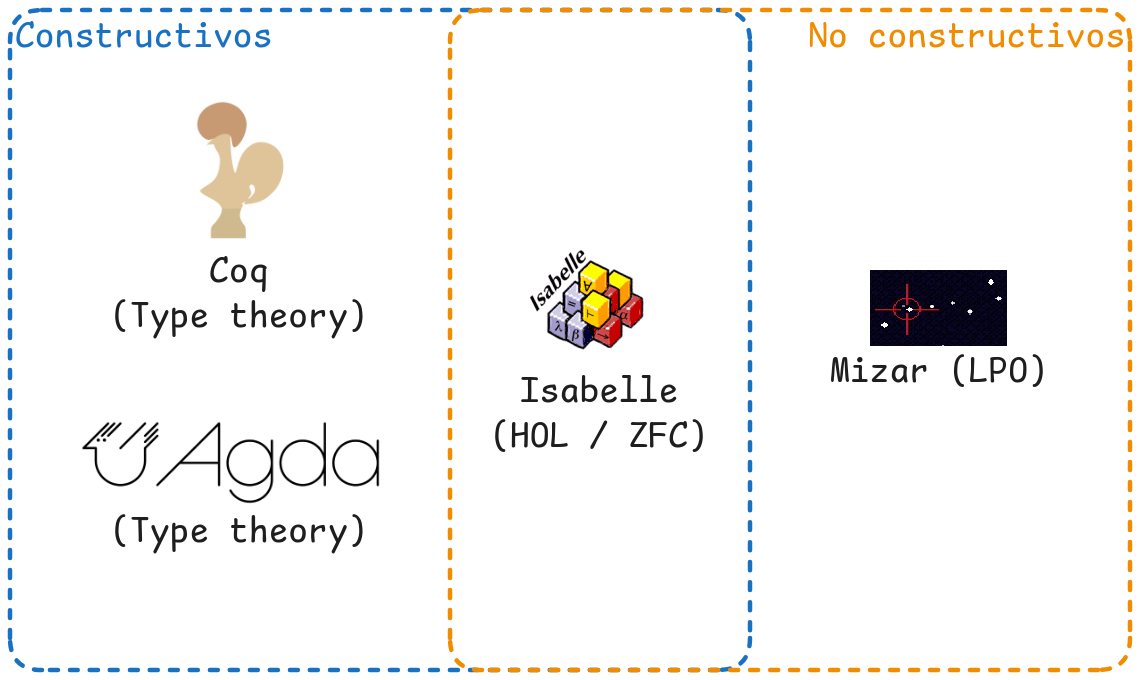
\includegraphics[scale=0.25]{img/ppt/proof-assistants.png}
    \end{figure}

    % De una demostración de una fórmula que afirma que existe un objeto que cumple con alguna propiedad, podemos encontrar tal objeto.
    \only<2>{
    \textbf{Extracción de testigos}: De una demo de
    $\exists \var . \pred(\var)$, encontrar $\term$ tq $\pred(\term)$.

    Lógica constructiva = sencillo, no constructiva = complicado.
    }
    \only<3>{
        \begin{center}
            ¿Dónde cae \ppaTool{}?
        \end{center}
    }
\end{frame}

\begin{frame}{PPA}
    \begin{figure}
        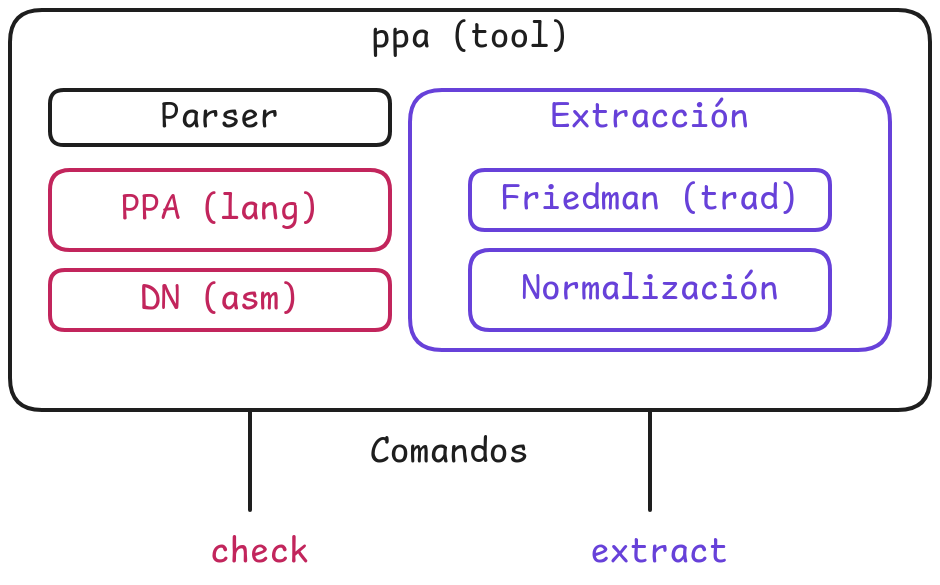
\includegraphics[scale=0.25]{img/ppt/ppa-tool-parts.png}
    \end{figure}
    Diseñamos e implementamos \ppaTool{} (\textit{Pani's Proof Assistant}). Partes:
    \begin{itemize}
        \item El lenguaje \textbf{PPA} para escribir demostraciones.
        \item Mecanismo de \textbf{extracción de testigos} de demostraciones no constructivas \alert{(aporte principal)}.
    \end{itemize}
\end{frame}

\begin{frame}{Ejemplo representación de demostraciones}
    \begin{definition}[Axiomas]
        \begin{enumerate}
            \item Los alumnos que faltan a los exámenes, los reprueban.
            \item Si se reprueba un final, se recursa la materia.
        \end{enumerate}
    \end{definition}
    \pause

    \begin{theorem}
        Si un alumno falta al final de una materia, entonces la recursa
    \end{theorem}
    \begin{proof}
        \begin{itemize}
    \item Asumo que falta. Quiero ver que recursa.
    \item Por (1), sabemos que si falta, entonces reprueba. Por lo tanto reprobó.
    \item Por (2), sabemos que si reprueba, entonces recursa. Por lo tanto recursó.
\end{itemize}
    \end{proof}
    \pause
    \begin{alertblock}{}
        \textbf{Problema}: Es poco precisa. No se puede representar formalmente.
    \end{alertblock}
\end{frame}

% \begin{frame}{Lógica de primer orden}
% Los predicados son \textbf{fórmulas atómicas}. Los de aridad 0 además son llamados \textit{variables proposicionales}.

% \begin{notation*}
%     Usamos
%     \begin{itemize}
%         \item $\var, \varTwo, \varThree, \dots$ como \textbf{variables}.
%         \item $\fun, \funTwo, \funThree, \dots$ como \textbf{símbolos de función}.
%         \item $\pred, \predTwo, \predThree, \dots$ como \textbf{símbolos de predicado}.
%         \item $\term, \termTwo, \dots$ para referirnos a \textbf{términos}.
%         \item $\formLit, \formLitTwo, \formLitThree, \dots$, $\form, \formTwo, \formThree, \dots$ y $\anyForm, \anyFormTwo, \dots$ para referirnos a \textbf{fórmulas}.
%     \end{itemize}
% \end{notation*}
% \end{frame}

\section{Deducción natural (DN)}


\begin{frame}{Lógica de primer orden}

    \begin{definition}[Términos]
        Los términos están dados por la gramática:
        \begin{align*}
            \term ::= &\ \var                               &\text{(variables)} \\
                      & \mid \fun(\term_1, \dots, \term_n) &\text{(funciones)}
        \end{align*}
    \end{definition}
    \begin{definition}[Fórmulas]
        Las fórmulas están dadas por la gramática:
        \begin{align*}
            \form, \formTwo ::=
             & \ \pred(\term_1, \dots, \term_n) & (\text{predicados})                \\
             & \mid \fFalse                     
               \mid \fTrue                      & \text{(falso y verdadero)} \\
             & \mid \form \fAnd \formTwo                        
               \mid \form \fOr \formTwo           & \text{(conjunción y disyunción)}     \\
             & \mid \form \fImp \formTwo                       
               \mid \fNot \form                 & \text{(implicación y negación)}                  \\
             & \mid \forall \var . \form        
               \mid \exists \var . \form        & \text{(cuantificador universal y existencial)}
        \end{align*}
    \end{definition}
    
\end{frame}

\begin{frame}{Reglas de inferencia}    
    Dos tipos para cada conectivo y cuantificador, dada una fórmula formada con un conectivo:
    \begin{itemize}
        \item \textbf{Introducción}: ¿Cómo la demuestro?
        \item \textbf{Eliminación}: ¿Cómo la uso para demostrar otra?
    \end{itemize}

    \begin{definition}[Reglas de inferencia]
        \proofTreeImpI
        \textit{Modus ponens:}
        \proofTreeImpE

        Donde $\ctx$ es un \textbf{contexto de demostración} y $\judG$ la \textbf{relación de derivabilidad} o consecuencia.
    \end{definition}
\end{frame}

\newcommand{\ctxColor}{\textcolor{Plum}{\ctx}}
% https://tex.stackexchange.com/questions/469229/show-up-only-parts-of-prooftree-on-beamer-frames
\begin{frame}{Ejemplo de demostración en DN}
    \begin{example}[Teorema en DN]
        Notamos:
        \begin{itemize}
            \item $\falta \equiv \predFalta(juan, \funFinal(logica))$
            \item $\reprueba \equiv \predReprueba(juan, \funFinal(logica))$
            \item $\recursa \equiv \predRecursa(juan, logica)$
        \end{itemize}
        Axiomas $\falta \fImp \reprueba$ y $\reprueba \fImp \recursa$.
        Afirmamos
        \(
            \falta \fImp \recursa.
        \)
    \end{example}
    \pause
    \begin{example}[Demostración en DN]
        \begin{prooftree}
        \AxiomC{}
        \RL{\uncover<5->{\alert<5>{\ruleAx}}}
        \only<-4>{\noLine}
        \UnaryInfC{\uncover<4->{$\ctxColor \judG \reprueba \fImp \recursa$}}
        %
        \AxiomC{}
        \RL{\uncover<6->{\alert{\ruleAx}}}
        \only<-5>{\noLine}
        \UnaryInfC{\uncover<6->{$\ctxColor \judG \falta \fImp \reprueba$}}
        \AxiomC{}
        \RL{\uncover<6->{\alert{\ruleAx}}}
        \only<-5>{\noLine}
        \UnaryInfC{\uncover<6->{$\ctxColor \judG \falta$}}
        \RL{\uncover<6->{\ruleImpE}}
        %
        \only<-5>{\noLine}
        \BinaryInfC{\uncover<4->{$\ctxColor \judG \reprueba$}}
        \RL{\uncover<4->{\ruleImpE}}
        \only<-3>{\noLine}
        \BinaryInfC{\uncover<3->{\(
            \ctxColor = 
                \alert<6>{(\falta \fImp \reprueba)},
                \alert<5>{(\reprueba \fImp \recursa)},
                \alert<6>{\falta}
            \judG
            \recursa 
            \)}}
        \RL{\uncover<3->{\ruleImpI}}
        \only<-2>{\noLine}
        \UnaryInfC{\(
            (\falta \fImp \reprueba), (\reprueba \fImp \recursa)
            \judG
                \falta \fImp \recursa
        \)}
        \end{prooftree}
    \end{example}
\end{frame}

% \begin{frame}{Deducción natural}
%     \begin{definition}[Contexto de demostración]
%         $\ctx$ es un \textbf{contexto de demostración}, conjunto de
%         fórmulas que se asumen válidas.

%         \textbf{Notación}: $\ctx, \anyForm = \ctx \cup \{\anyForm\}$
%     \end{definition}
%     \pause
%     \begin{definition}[Relación de derivabilidad]
%         \begin{itemize}
%             \item $\judG$ es la \textbf{relación de derivabilidad} definida a
%             partir de las \textit{reglas de inferencia}.
%             \item Permite escribir
%             juicios $\ctx \judG \anyForm$. Intuición: \textit{``$\anyForm$ es
%             una consecuencia de las suposiciones de $\ctx$''}
%             \item Es cierto si en una cantidad finita de
%             pasos podemos concluir $\anyForm$ a partir de las fórmulas de
%             $\ctx$, los axiomas y las reglas de inferencia.
%         \end{itemize}
%     \end{definition}
% \end{frame}



\begin{frame}{Reglas de inferencia}
    Otras reglas de inferencia
    \begin{itemize}
        \item \ruleNotI, \ruleNotE, \ruleAndI, \ruleAndEOne, \ruleAndETwo
        \item \ruleOrIOne, \ruleOrITwo, \ruleOrE
        \item \ruleForallI, \ruleForallE, \ruleExistsI, \ruleExistsE
        \item \ruleFalseE, \ruleTrueI, \ruleLEM
    \end{itemize}
    \pause
    \begin{block}{Reglas admisibles}
        No tenemos regla por ej. para \textit{modus tollens}:
        \[
            \big((\form \fImp \formTwo) \fAnd \fNot \formTwo\big) \fImp \fNot \form
        \]
        \vspace{-\baselineskip}
        \begin{itemize}
            \item Queremos un sistema lógico \textbf{minimal}, sin reglas \textbf{admisibles}.
            \item Se implementan como funciones o \textit{macros}.
        \end{itemize}    
    \end{block}
    % \pause
    % \begin{block}{Alfa equivalencia}
    %     \begin{itemize}
    %         \item Podemos usar $\exists \var . \pred(\var)$ y $\exists \varTwo . \pred(\varTwo)$ de forma intercambiable.
    %         \item Son $\alpha$-equivalentes (renombrando variables ligadas de forma apropiada, son iguales).
    %     \end{itemize}
    % \end{block}
\end{frame}

% \begin{frame}{Reglas admisibles}
%     \begin{itemize}
%         \item Mencionamos \textit{modus tollens} pero no aparece en las reglas de inferencia.
        
%     \end{itemize} 
%     \pause
%     \begin{lemma}[Modus tollens]
        
%     \begin{prooftree}
%         \AxiomC{}
%         \RL{\ruleAx}
%         \UnaryInfC{\(\ctx \judG (\form \fImp \formTwo) \fAnd \fNot \formTwo\)}
%         \RL{\ruleAndETwo}
%         \UnaryInfC{\(
%             \ctx \judG \fNot \formTwo
%         \)}
%         \AxiomC{}
%         \RL{\ruleAx}
%         \UnaryInfC{\(\ctx \judG (\form \fImp \formTwo) \fAnd \fNot \formTwo\)}
%         \RL{\ruleAndEOne}
%         \UnaryInfC{$\ctx \judG \form \fImp \formTwo$}
%         \AxiomC{}
%         \RL{\ruleAx}
%         \UnaryInfC{$\ctx \judG \form$}
%         \RL{\ruleImpE}
%         \BinaryInfC{\(
%             \ctx \judG \formTwo
%         \)}
%         \RL{\ruleNotE{}}
%         \BinaryInfC{\(
%             \ctx = (\form \fImp \formTwo) \fAnd \fNot \formTwo, \form
%             \judG
%             \fFalse
%         \)}
%         \RL{\ruleNotI{}}
%         \UnaryInfC{\(
%             (\form \fImp \formTwo) \fAnd \fNot \formTwo
%             \judG
%             \fNot \form
%         \)}
%         \RL{\ruleImpI{}}
%         \UnaryInfC{\(\judG
%             (\form \fImp \formTwo \fAnd \fNot \formTwo)
%             \fImp \fNot\form
%         \)}
%     \end{prooftree}
%     \end{lemma}
% \end{frame}

%\begin{frame}{Sustitución}
    % \begin{definition}[Sustitución]
    %     $\form \subst{\var}{\term}$ sustituir todas las
    %     ocurrencias libres de la variable $\var$ por el término $\term$ en la
    %     fórmula $\form$.
    % \end{definition}
    % \pause
    % \begin{block}{Capturas}
    %     Evitamos automáticamente la \textbf{captura de variables} (renombrando a fórmula $\alpha$-equivalente tq no ocurra)
    %     \begin{align*}
    %     (\forall \varTwo . \pred(\bm{\var}, \varTwo))\subst{\var}{\varTwo} &\not =
    %     \forall \varTwo . \pred(\alert{\varTwo}, \varTwo) & & \text{(capturada)}\\
    %     (\forall \varTwo . \pred(\bm{\var}, \varTwo))\subst{\var}{\varTwo} &=
    %     \forall \alert{\varThree} . \pred(\bm{\varTwo}, \alert{\varThree}) & & \text{(renombrada)}
    %     \end{align*}
    % \end{block}
%\end{frame}

%\begin{frame}{Alfa equivalencia}
    % \begin{itemize}
    %     \item Algoritmo naíf: cuadrático en la estructura de la fórmula,
    %     renombrando recursivamente.
    %     \item Algoritmo cuasilineal: manteniendo dos sustituciones, una por
    %     fórmula.
    % \end{itemize}
    % \begin{example}
    %     \begin{align*}
    %         (\exists \var . \fun(\var)) &\alphaEq (\exists \varTwo . \fun(\varTwo))
    %         &&\{\}, \{\}
    %         \\
    %         &\iff \fun(\var) \alphaEq \fun(\varTwo)
    %             &&\{\var \mapsto \varThree\}, \{\varTwo \mapsto \varThree\}\\
    %         &\iff \var \alphaEq \varTwo
    %             &&\{\var \mapsto \varThree\}, \{\varTwo \mapsto \varThree\}\\
    %         &\iff \varThree = \varThree.
    %     \end{align*}        
    % \end{example}
%\end{frame}

\section{PPA}

\begin{frame}{Mathematical Vernacular}
    \begin{center}
        Mizar $\rightsquigarrow$
        Isar (Isabelle) $\rightsquigarrow$
        \textit{Mathematical
        Vernacular}\footnote{De Freek Wiedijk}
    \end{center}
    

    Forma \textit{natural} de representar demostraciones matemáticas. Ideas:
    \pause
    \begin{itemize}[<+->]
        \item \textbf{Deducción natural en estilo de \textit{Fitch}}.
        \item \textbf{Reglas de inferencia \textit{declarativas}}:
         \[\form_1, \dots, \form_n \judG \form\]
        \item \textbf{Sintaxis similar a un lenguaje de programación}
    \end{itemize}
\end{frame}

\begin{frame}[fragile]{PPA}
    \textit{Lenguaje} PPA, inspirado en el
    \textit{Mathematical Vernacular}.
    \onslide<1->{\lstinputlisting[title=Ejemplo demostración,lastline=4]{listings/ppt/alumnos-corto.ppa}}\vspace*{-\baselineskip}

    \onslide<2->{\lstinputlisting[firstnumber=last,firstline=5,lastline=8]{listings/ppt/alumnos-corto.ppa}}\vspace*{-\baselineskip}
    \onslide<3->{\lstinputlisting[firstnumber=last,firstline=9,lastline=10]{listings/ppt/alumnos-corto.ppa}}\vspace*{-\baselineskip}
    \onslide<4->{\lstinputlisting[firstnumber=last,firstline=11,lastline=11]{listings/ppt/alumnos-corto.ppa}}\vspace*{-\baselineskip}
    \onslide<5->{\lstinputlisting[firstnumber=last,firstline=12,lastline=12]{listings/ppt/alumnos-corto.ppa}}\vspace*{-\baselineskip}
    \onslide<6->{\lstinputlisting[firstnumber=last,firstline=13]{listings/ppt/alumnos-corto.ppa}}\vspace*{-\baselineskip}
\end{frame}


% \begin{frame}[fragile]{Identificadores}
%     \begin{itemize}
%         \item \textbf{Variables} (\lstinline{<var>})
%         \begin{center}
%             \verb/(\_|[A-Z])[a-zA-Z0-9\_\-]*(\')*/
%         \end{center}
%         \item \textbf{Identificadores} (\lstinline{<id>})
%         \begin{center}
%             \verb/[a-zA-Z0-9\_\-\?!#\$\%\*\+\<\>\=\?\@\^]+(\')*/
%         \end{center}
%         \item \textbf{Nombres} (\lstinline{<name>})
        
%         Pueden ser identificadores o strings arbitrarios encerrados por comillas dobles.
%         \begin{center}
%             \verb/<id> | \"[^\"]*\"/
%         \end{center}
%     \end{itemize}
% \end{frame}

% \begin{frame}[fragile]{Programas}
%     Un \textbf{programa} de PPA consiste en una lista de \textbf{declaraciones},
%     que pueden ser
%     \begin{itemize}
%         \item \textbf{Axiomas}: fórmulas que se asumen válidas
%         \begin{lstlisting}[numbers=none]
% axiom <name> : <form>
%         \end{lstlisting}
%         \item \textbf{Teoremas}: fórmulas junto con sus demostraciones.
% \begin{lstlisting}[numbers=none]
% theorem <name> : <form>
% proof
%     <steps>
% end
% \end{lstlisting}
%     \end{itemize}
% \end{frame}

% \begin{frame}[fragile]{Fórmulas y términos}
%     Términos:
%     \begin{itemize}
%         \item Variables: \lstinline{<var>}
%         \item Funciones: \lstinline{<id>(<term>, ..., <term>)}
%     \end{itemize}

%     Funciones:
%     \begin{itemize}
%         \item Predicados: \lstinline{<id>(<term>, ..., <term>)}
%         \item \lstinline{<form> & <form>}
%         \item \lstinline{<form> | <form>}
%         \item \lstinline{<form> -> <form>}
%         \item \lstinline{<form> <-> <form>}
%         \item \lstinline{~ <form>}
%         \item \lstinline{exists <var> . <form>}
%         \item \lstinline{forall <var> . <form>}
%         \item \lstinline{true}, \lstinline{false}
%         \item \lstinline{(<form>)}
%     \end{itemize}
% \end{frame}

% \begin{frame}{Demostraciones}
%     \begin{columns}
%         \begin{column}{0.5\textwidth}
%             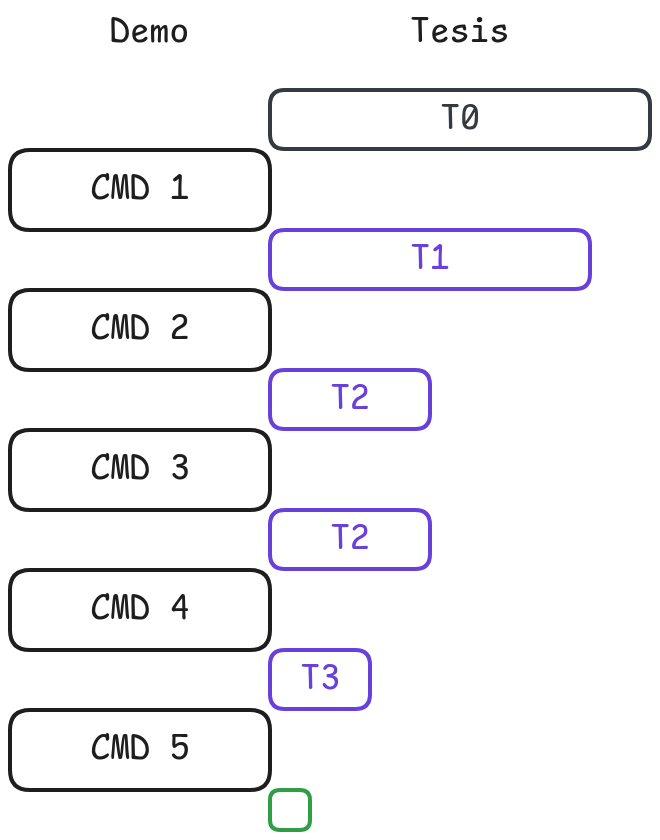
\includegraphics[scale=0.25]{img/ppt/dem-reduccion.png}
%         \end{column}
%         \begin{column}{0.5\textwidth}
%             Lista de \textbf{comandos} que reducen sucesivamente la \textit{tesis} (fórmula a demostrar) hasta agotarla.
%         \end{column}
%     \end{columns}
% \end{frame}

% \begin{frame}[fragile]{Thus y Have}
%     \begin{command}
%     \lstinline{thus <form> by <h1>, ..., <hn>}

%     \vspace{0.25cm}

%     Si \lstinline{<form>} es \textit{parte} de la tesis, y el \textit{solver} puede demostrar la implicación, lo demuestra automáticamente y lo descarga de la tesis.
%     \end{command}

%     \vspace{0.25cm}

%     \begin{command}
%         \lstinline{have <name>: <form> by <h1>, ..., <hn>}
    
%         \vspace{0.25cm}
    
%         Análogo a \lstinline{thus}, pero introduce una afirmación \textit{auxiliar}
%         sin reducir la tesis, agregándola al contexto.
%     \end{command}    
    % \vspace{-0.4cm}
    % \begin{columns}[t]
    %     \begin{column}{0.5\textwidth}
    %         \lstinputlisting[title=Eliminación de implicación]{listings/interfaz/by-imp.ppa}
    %     \end{column}
    %     \begin{column}{0.5\textwidth}
    %         \lstinputlisting[title=Eliminación de universal]{listings/interfaz/by-forall.ppa}
    %     \end{column}
    % \end{columns}

%\end{frame}

% \begin{frame}[fragile]{Have}
%     \pause
%     \begin{block}{Hipótesis anterior implícita}
%         Ambas pueden referirse a la hipótesis anterior con guión medio
%         (\lstinline{-}), y pueden hacerlo implícitamente usando \lstinline{hence} y
%         \lstinline{then}.
    
%         \begin{table}[H]
%             \centering
%         \begin{tabular}{l|l|l}
%         Comando             & Alternativo             & ¿Reduce la tesis? \\
%         \hline
%         \lstinline|thus|    & \lstinline|hence|       & Sí               \\
%         \lstinline|have|    & \lstinline|then|        & No              
%         \end{tabular}
%         \end{table}    
%     \end{block}
%     % \begin{figure}[H]
%     %     \centering
%     %     \small Eliminación de implicación en dos pasos
        
%     %     \begin{tabular}{c}
%     %         \lstinputlisting{listings/interfaz/by-imp-have.ppa}
%     %     \end{tabular}
%     % \end{figure}
%     % \begin{columns}
%     %     \begin{column}{0.5\textwidth}
%     %     \lstinputlisting[
%     %         firstline=1,
%     %         lastline=9,
%     %         title=Eliminación en dos pasos,
%     %     ]{listings/interfaz/by-imp-then.ppa}
%     %     \end{column}
%     %     \begin{column}{0.5\textwidth}
%     %         \lstinputlisting[
%     %             linerange={12-16, 19-23},
%     %             numbers=none,
%     %             title=Alternativas equivalentes,
%     %         ]{listings/interfaz/by-imp-then.ppa}
%     %     \end{column}
%     % \end{columns}

% \end{frame}
% \begin{frame}[fragile]{By opcional}
%     \begin{itemize}
%         \item El \lstinline{by} es opcional
%         \item Si se omite, la fórmula debe ser
%         demostrable por el \textit{solver} sin partir de ninguna hipótesis
%         \item Vale para todas las tautologías proposicionales.
%     \end{itemize}

%     \begin{figure}[H]
%         \centering
%         \small Tautología proposicional
        
%         \begin{tabular}{c}
%             \lstinputlisting{listings/interfaz/by-taut.ppa}
%         \end{tabular}
%     \end{figure}
% \end{frame}

\begin{frame}{Comandos y reglas de inferencia}
    \begin{columns}
        \begin{column}{0.5\textwidth}
            \begin{table}[H]
                \centering
                \begin{tabular}{c|c}
                Regla & Comando \\
                \hline
                \ruleLEM        &   \lstinline|cases| \\
                \ruleAx         &   \lstinline|by| \\
                \ruleExistsI    &   \lstinline|take| \\
                \ruleExistsE    &   \lstinline|consider| \\
                \ruleForallI    &   \lstinline|let| \\
                \ruleForallE    &   \lstinline|by| \\
                \ruleOrIOne     &   \lstinline|by| \\
                \ruleOrITwo     &   \lstinline|by| \\
                \ruleOrE        &   \lstinline|cases|
                \end{tabular}
            \end{table}
        \end{column}
        \begin{column}{0.5\textwidth}
            \begin{table}[H]
                \centering
                \begin{tabular}{c|c}
                Regla & Comando \\
                \hline
                \ruleAndI       &   \lstinline|by| \\
                \ruleAndEOne    &   \lstinline|by| \\
                \ruleAndETwo    &   \lstinline|by| \\
                \ruleImpI       &   \lstinline|suppose| \\
                \ruleImpE       &   \lstinline|by| \\
                \ruleNotI       &   \lstinline|suppose| \\
                \ruleNotE       &   \lstinline|by| \\
                \ruleTrueI      &   \lstinline|by| \\
                \ruleFalseE     &   \lstinline|by|
                \end{tabular}
            \end{table}
        \end{column}
    \end{columns}
    \pause
    Adicionales:
    \begin{itemize}
        \item \lstinline{equivalently}: Reduce la tesis a una fórmula equivalente.
        \item \lstinline{claim}: Análogo a \lstinline{have} pero con una sub-demostración.
    \end{itemize}
\end{frame}

% \begin{frame}[fragile]{Suppose (\ruleImpI / \ruleNotI)}
%     \begin{command}
%         \lstinline{suppose <name>: <form>} \quad (\ruleImpI / \ruleNotI)
%     \end{command}

%     \begin{itemize}
%         \item  Si la tesis es una implicación $\form \fImp \formTwo$, agrega el antecedente
%         $\form$ como hipótesis con el nombre dado y reduce la tesis al consecuente
%         $\formTwo$
%         \item Viendo la negación como una implicación $\fNot \form \equiv
%         \form \fImp \fFalse$, permite introducir negaciones, tomando
%         $\formTwo = \fFalse$.
%     \end{itemize}

%     \begin{columns}
%         \begin{column}{0.5\textwidth}
%             \lstinputlisting[
%                 firstline=1, lastline=7,
%                 title=Introducción de implicación,
%             ]{listings/interfaz/suppose.ppa}
%         \end{column}
%         \begin{column}{0.5\textwidth}
%             \lstinputlisting[
%                 firstline=9, lastline=15,
%                 title=Introducción de negación,
%             ]{listings/interfaz/suppose.ppa}    
%         \end{column}
%     \end{columns}
% \end{frame}

% \begin{frame}[fragile]{Cases (\ruleOrE)}
%     \begin{command}
%         \lstinline{cases by <h1>, ..., <hn>} \quad (\ruleImpI / \ruleNotI)
%     \end{command}
%     \begin{columns}
%         \begin{column}{0.5\textwidth}
%         \begin{itemize}
%             \item Permite razonar por casos a partir de una disyunción. Para cada uno, se debe
%             demostrar la tesis en su totalidad.
%             \item Si los casos son \lstinline{<f1>} a
%             \lstinline{<fn>}, tiene que valer \lstinline{<f1> | ... | <fn> by} \lstinline{<h1>, ..., <hn>}.
%             \item Se puede omitir el \lstinline{by} para razonar mediante LEM (casos $\anyForm$ y $\fNot \anyForm$).
%         \end{itemize}
%         \end{column}
%         \begin{column}{0.5\textwidth}
%             \lstinputlisting[
%         title=Cases,
%         firstline=1, lastline=11,
%     ]{listings/interfaz/cases.ppa}
%         \end{column}
%     \end{columns}
% \end{frame}

% \begin{frame}[fragile]{Take (\ruleExistsI)}
%     \begin{command}
%         \lstinline{take <var> := <term>} \quad (\ruleExistsI)
%     \end{command}
%     \vfill
%     \begin{itemize}
%         \item Introduce un existencial instanciando su variable y reemplazándola por un término.
%         \item Si la tesis es \lstinline{exists X . p(X)}, luego de \lstinline{take X := a}, se reduce a \lstinline{p(a)}.
%     \end{itemize}
% \end{frame}

% \begin{frame}[fragile]{Consider (\ruleExistsE)}
%     \begin{command}
%         \lstinline{consider <var> st <name>: <form> by <h1>, ..., <hn>} \quad (\ruleExistsE)
%     \end{command}
%     \begin{itemize}
%         \item Si se puede justificar \lstinline{exists X. p(X)}, permite razonar sobre tal \lstinline{X}.
%         \item Agrega \lstinline{<form>} como hipótesis al contexto, con nombre \lstinline{<name>}. No reduce la tesis.
%         \item Debe valer \lstinline{exists <var> . <form> by <h1>, ..., <hn>}
%         \item Permite $\alpha$-equivalencias: Si podemos justificar \lstinline{exists X. p(X)}, podemos usarlo como \lstinline{consider Y st h: p(Y) by ...}.
%     \end{itemize}
% \end{frame}

% \begin{frame}[fragile]{Let (\ruleForallI)}
%     \begin{command}
%         \lstinline{let <var>} \quad (\ruleForallI)
%     \end{command}
%     \begin{itemize}
%         \item Permite demostrar un cuantificador universal.
%         \item Si la tesis es \lstinline{forall X . p(X)}, luego de \lstinline{let X}, la tesis se reduce a \lstinline{p(X)}.
%         \item Permite renombrar la variable, por ejemplo luego de \lstinline{let Y} la tesis se reduce a \lstinline{p(Y)}.
%     \end{itemize}
% \end{frame}

% \begin{frame}[fragile]{Comandos adicionales}
%     \begin{command}
%         \lstinline{equivalently <form>}

%         Permite reducir la tesis a una fórmula equivalente
%     \end{command}

%     \begin{command}
%         \lstinline{claim <name>: <form>}

%         Análogo a \lstinline{have} pero con una sub-demostración.
%     \end{command}

%     \begin{lstlisting}[numbers=none, title=Esquema de claim]
% theorem t: <form1>
% proof
%     claim <name>: <form2>
%     proof
%         // Demostración de <form2>.
%     end
%     // Demostración de <form1> refiriéndose a <name>.
% end
%     \end{lstlisting}

%     \begin{itemize}
%         \item Permite reducir la tesis a una fórmula equivalente
%         \item Se puede usar por ejemplo para descarga de conjunciones, o para razonar por el absurdo mediante la eliminación de la doble negación.
%     \end{itemize}

%     \begin{columns}
%         \begin{column}{0.5\textwidth}
%             \lstinputlisting[title=Descarga de conjunción]{listings/interfaz/equivalently.ppa}
%         \end{column}
%         \begin{column}{0.5\textwidth}
% \begin{lstlisting}[numbers=none,title=Razonamiento por el absurdo]
% theorem t: <form>
% proof
%     equivalently ~~<form>
%     suppose <name>: ~<form>
%     // Demostración de <form>
%     // por el absurdo,
%     // asumiendo ~<form>
%     // y llegando a una
%     // contradicción (false).
% end
% \end{lstlisting}
%         \end{column}
%     \end{columns}
%\end{frame}

\begin{frame}{Certificados}
    \begin{columns}
        
        \begin{column}{0.5\textwidth}
            \begin{itemize}
                \item Las demostraciones de \ppaLang{} se \textbf{certifican} generando
                una demostración de deducción natural.
                \item Evita confiar en la implementación del asistente.
                \onslide<2->{
                \item Cumple con el \textbf{Criterio de de Bruijn}
                }
            \end{itemize}
        \end{column}
        \begin{column}{0.5\textwidth}
            \begin{figure}
                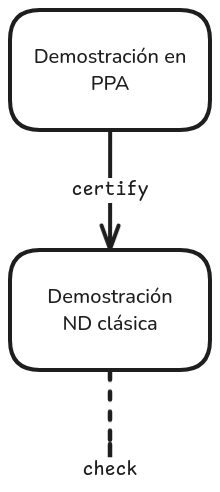
\includegraphics[scale=0.35]{img/ppt/certify.png}
            \end{figure}
        \end{column}
    \end{columns}
    % \pause
    % \begin{block}{Criterio de de Bruijn}
    %     Un asistente de demostración cumple con el criterio de de Bruijn si
    %     satisface que sus demostraciones puedan ser chequeadas por un programa
    %     independiente, pequeño y confiable.
    % \end{block}
\end{frame}


\begin{frame}[fragile]{Certificado de demostraciones}
    El procedimiento de certificado de una demostración es recursivo:
    % se certifica cada comando, generando una demostración en deducción natural cuyas premisas son el certificado del resto de la demostración en PPA.
    \begin{figure}
        \begin{columns}
            \begin{column}{0.45\textwidth}
                \begin{tabular}{c}
                    \lstinputlisting{listings/ppt/certificado.ppa}
                \end{tabular}
    
            \end{column}
            \begin{column}{0.35\textwidth}
                \begin{prooftree}
                    \AxiomC{}
                    \RL{\alert{\ruleAxh{h}}}
                    \UnaryInfC{$h: p(v) \judG p(v)$}
                    \RL{\ruleExistsI}
                    \UnaryInfC{$h: p(v) \judG \exists x . p(X)$}
                    \RL{\ruleImpIh{h}}
                    \UnaryInfC{$\judG p(v) \fImp \exists x . p(X)$}
                \end{prooftree}
            \end{column}
        \end{columns}
    \end{figure}
    \pause
    \begin{center}
        \begin{minted}{haskell}
            PImpI
                { hypAntecedent = "h"
                , proofConsequent =
                    PExistsI
                        { inst = TFun "v" []
                        , proofFormWithInst = PAx "h"
                        }
                }
                \end{minted}
            
    \end{center}
\end{frame}



% \begin{frame}{Contexto global}
%     Se generan $N$ demostraciones de deducción natural para cada programa, y se guardan en el \textit{contexto global}. El chequeo se extiende a contextos.
    
%     \begin{figure}
%         \begin{columns}
%             \begin{column}{0.4\textwidth}
%                 \begin{tabular}{c}
%                     \lstinputlisting{listings/certifier/two-theorems.ppa}
%                 \end{tabular}
%             \end{column}
%             \begin{column}{0.3\textwidth}
%                 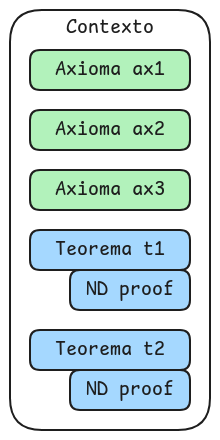
\includegraphics[scale=0.4]{img/ppa-context.png}
%             \end{column}
%         \end{columns}
%         \caption{Contexto resultante de certificar un programa}
%     \end{figure}
% \end{frame}


% \begin{frame}{Contexto local}
%     Cada demostración tiene un contexto local a ella con las hipótesis agregadas por ciertos comandos (\lstinline{suppose}, \lstinline{consider}, \lstinline{have}, \lstinline{claim}, etc.).

%     \begin{figure}[h]
%         \centering
%         \begin{columns}
%             \begin{column}{0.5\textwidth}
%                 \begin{tabular}{c}
%                     \lstinputlisting{listings/certifier/local-context.ppa}
%                 \end{tabular}
%             \end{column}
%             \begin{column}{0.35\textwidth}
%                 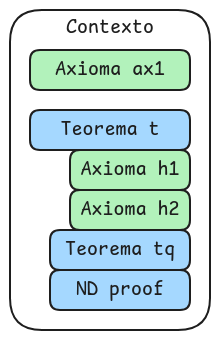
\includegraphics[scale=0.33]{img/ppa-local-context.png}
%             \end{column}
%         \end{columns}
%         \caption{Ejemplo de contexto local}
%     \end{figure}
% \end{frame}

\begin{frame}{Ejemplo sin cuantificadores (1/4)}
    \begin{figure}
        \centering
        \small By sin cuantificadores

        \vspace{0.1cm}
        \begin{tabular}{c}
            \lstinputlisting{listings/certifier/by-modus-ponens.ppa}
        \end{tabular}
    \end{figure}
    \pause
    \begin{enumerate}
        \item Para certificar \lstinline{thus b by ax1, ax2} hay que generar una
        demostración para la implicación \[
            \ctx \judG \big((a \fImp b) \wedge a \big) \fImp b
        \]

        tomando las hipótesis \lstinline{ax1, ax2} del \textbf{contexto}.
    \end{enumerate}
\end{frame}

\begin{frame}{Ejemplo sin cuantificadores (2/4)}
    \begin{enumerate}
        \setcounter{enumi}{1}
        \item \textbf{Razonamos por el absurdo}: Negamos la fórmula y buscamos una contradicción.
        \[ 
            \ctx, \fNot [ \big( (a \to b) \fAnd a \big) \to b ] \judG \fFalse
        \]
    \end{enumerate}
    \pause
    \begin{definition}[Eliminación de doble negación]
        \[
            \AxiomC{}
            \RL{\ruleDnegE}
            \admissibleRuleLine
            \UnaryInfC{$\fNot \fNot \form \judG \form$}            
            \DisplayProof               
            %
            \quad\equiv\quad
            \AxiomC{}
            \RL{\ruleLEM}
            \UnaryInfC{$\judg{\ctx}{\form \vee \neg \form}$}
            \DisplayProof
        \]
    \end{definition}
\end{frame}

% \begin{frame}{Contradicciones}
%     \begin{exampleblock}{Ejemplo}
%     \begin{prooftree}
%         \def\defaultHypSeparation{\hskip .1in}
%         \AxiomC{}
%         \LL{\ruleAx}
%         \UnaryInfC{\(
%             \ctx \judG
%             \begin{aligned}[b]
%                 &(\fNot a \fAnd a \fAnd \fNot b)\\
%                 &\vee (b \fAnd a \fAnd \fFalse)
%             \end{aligned}
%         \)}
%         \AxiomC{$\someProof_L$}
%         \noLine
%         \UnaryInfC{\(
%             \ctx, \fNot a \fAnd a \fAnd \fNot b \judG \fFalse
%         \)}
%         \AxiomC{}
%         \RL{\ruleAx}
%         \UnaryInfC{$\ctx_1 \judG b \fAnd a \fAnd \fFalse$}
%         \RL{\ruleAndEProj{\fFalse}}
%         \admissibleRuleLine
%         \UnaryInfC{\(
%             \ctx, b \fAnd a \fAnd \fFalse \judG \fFalse
%         \)}
%         \RL{\ruleOrE}
%         \TrinaryInfC{\(
%             \ctx = (\fNot a \fAnd a \fAnd \fNot b)
%             \vee
%             (b \fAnd a \fAnd \fFalse)
%             \judG
%             \fFalse
%         \)}
%     \end{prooftree}
    
%     donde
    
%     \begin{prooftree}
%         \AxiomC{}
%         \RL{\ruleAx}
%         \UnaryInfC{$\ctx_1 \judG \fNot a \fAnd a \fAnd \fNot b$}
%         \RL{\ruleAndEProj{\fNot a}}
%         \admissibleRuleLine
%         \UnaryInfC{$\ctx_1 \judG \fNot a$}
%         \AxiomC{}
%         \RL{\ruleAx}
%         \UnaryInfC{$\ctx_1 \judG \fNot a \fAnd a \fAnd \fNot b$}
%         \RL{\ruleAndEProj{a}}
%         \admissibleRuleLine
%         \UnaryInfC{$\ctx_1 \judG a$}
%         \RL{\ruleNotE}
%         \LL{$\someProof_L=$}
%         \BinaryInfC{\(
%             \ctx_1 = \ctx, b \fAnd a \fAnd \fFalse \judG \fFalse
%         \)}
%     \end{prooftree}
%     \end{exampleblock}
%     \pause
%     \begin{lemma}[Regla admisible \ruleAndEProj{\anyForm}]
%         \begin{prooftree}
%             \AxiomC{$\ctx \judG \anyForm_1 \fAnd \dots \fAnd \anyForm_i \fAnd \dots \fAnd \anyForm_n$}
%             \AxiomC{$n \in \setNaturals$}
%             \admissibleRuleLine
%             \RL{\ruleAndEProj{\anyForm_{i}}}
%             \BinaryInfC{$\ctx \judG \anyForm_i$}
%         \end{prooftree}
%     \end{lemma}
% \end{frame}

\begin{frame}{Ejemplo sin cuantificadores (2/3)}
    \begin{enumerate}[<+->]
        \setcounter{enumi}{2}
        \item La convertimos a \textbf{DNF} (\textit{Forma Normal Disyuntiva})
        \begin{align*}
            &\fNot [ \big( (a \to b) \fAnd a \big) \to b ] \\
            &\equiv \fNot [ \fNot \big( (a \to b) \fAnd a \big) \fOr b ]
                && \just{\form \to \formTwo \equiv \fNot \form \fOr \formTwo}\\
            &\equiv \fNot \fNot \big( (a \to b) \fAnd a \big) \fAnd \fNot b
                && \just{\fNot(\form \fOr \formTwo) \equiv \fNot \form \fAnd \fNot \formTwo}\\
            &\equiv \big( (a \to b) \fAnd a \big) \fAnd \fNot b
                && \just{\fNot\fNot \form \equiv \form}\\
            &\equiv (\fNot a \fOr b) \fAnd a \fAnd \fNot b
                 && \just{\form \to \formTwo \equiv \fNot \form \fOr \formTwo}\\
            &\equiv (\fNot a \fOr b) \fAnd a \fAnd \fNot b
                && \just{(\form \fOr \formTwo) \fAnd \formThree \equiv (\form \fAnd \formThree) \fOr (\formTwo \fAnd \formThree)}\\
            &\equiv \begin{aligned}[t]
                &\bm{(\fNot a \fAnd a \fAnd \fNot b)}\ \bm{\vee}\\
                &\bm{(b \fAnd a \fAnd \fNot b)}
            \end{aligned}
        \end{align*}
    \end{enumerate}
\end{frame}

% \begin{frame}{Conversión a DNF}
%     Implementamos una traducción mediante el siguiente sistema de reescritura. \textbf{Algoritmo}: reescribir de a un paso hasta que no cambie (clausura de Kleene)
%         \begin{align*}
%             \fNot\fNot \formLit &\rewrite
%                 \formLit
%                 &&\text{eliminación de $\fNot\fNot$}\\
%             \fNot \fFalse &\rewrite
%                 \fTrue\\
%             \fNot \fTrue &\rewrite
%                 \fFalse\\
%             \formLit \fImp \formLitTwo &\rewrite
%                 \fNot \formLit \fOr \formLitTwo
%                 &&\text{definición de implicación}\\
%             \fNot(\formLit \fOr \formLitTwo) &\rewrite
%                 \fNot \formLit \fAnd \fNot \formLitTwo
%                 &&\text{distributiva de $\fNot$ sobre $\fAnd$}\\
%             \fNot(\formLit \fAnd \formLitTwo) &\rewrite
%                 \fNot \formLit \fOr \fNot \formLitTwo
%                 &&\text{distributiva de $\fNot$ sobre $\fOr$}\\
%             (\formLit \fOr \formLitTwo) \fAnd \formLitThree &\rewrite
%                 (\formLit \fAnd \formLitThree) \fOr (\formLitTwo \fAnd \formLitThree)
%                 &&\text{distributiva de $\fAnd$ sobre $\fOr$ (der)}\\
%             \formLitThree \fAnd (\formLit \fOr \formLitTwo) &\rewrite
%                 (\formLitThree \fAnd \formLit) \fOr (\formLitThree \fAnd \formLitTwo)
%                 &&\text{distributiva de $\fAnd$ sobre $\fOr$ (izq)}\\
%             \formLit \fOr (\formLitTwo \fOr \formLitThree) &\rewrite
%                 (\formLit \fOr \formLitTwo) \fOr \formLitThree
%                 &&\text{asociatividad de $\fOr$}\\
%             \formLit \fAnd (\formLitTwo \fAnd \formLitThree) &\rewrite
%                 (\formLit \fAnd \formLitTwo) \fAnd \formLitThree
%                 &&\text{asociatividad de $\fAnd$}
%         \end{align*}
% \end{frame}

% \begin{frame}{Conversión a DNF - Congruencias}
%     Para reescribir una sub-fórmula (trivial sintácticamente), hay que demostrar las congruencias de los conectivos.
%     \[
%         \formLit \fOr \alert<1,2>{\fNot (\formLitTwo \fOr \formLitThree)}
%         \judG
%         \formLit \fOr \alert<1,2>{(\fNot \formLitTwo \fAnd \fNot \formLitThree)}
%     \]\pause
%     \vspace{-0.3cm}
%     \begin{block}{Congruencias}
%         \vspace{-0.3cm}
%         \begin{gather*}
%         \form \judG \form'
%         \Rightarrow \form \fAnd \formTwo \judG \form' \fAnd \formTwo
%         \qquad
%         \formTwo \judG \formTwo'
%         \Rightarrow \form \fAnd \formTwo \judG \form \fAnd \formTwo'
%         \\
%         \form \judG \form'
%         \Rightarrow \form \fOr \formTwo \judG \form' \fOr \formTwo
%         \qquad
%         \alert<2>{\formTwo \judG \formTwo'
%         \Rightarrow \form \fOr \formTwo \judG \form \fOr \formTwo'}
%         \\
%         \alert<3->{\form'} \judG \form
%         \Rightarrow \fNot \form \judG \fNot \alert<3->{\form'}
%         \end{gather*}        
%     \end{block}
%     \pause
%     \begin{alertblock}{$\fNot$ es contravariante}
%         Para demostrar $\fNot \form \judG \fNot \form'$ no necesitamos una demostración de $\form \judG \form'$ (\textit{covariante}), sino de $\form' \judG \form$ (\textit{contravariante}).
%         \pause

%         $\Rightarrow$ para todas las reescrituras, incluso las congruencias, tenemos que demostrarlas en ambos sentidos.
%     \end{alertblock}
% \end{frame}

\begin{frame}{Conversión a DNF - Reglas admisibles}
    \begin{block}{Reglas admisibles para conversión a DNF}
        \begin{columns}[t]
        \begin{column}{0.5\textwidth}
            \centering
            \textbf{Pasos base}
            \begin{align*}
            \fNot\fNot \formLit &\judgEquiv
                \formLit
                \\
            \fNot \fFalse &\judgEquiv
                \fTrue\\
            \fNot \fTrue &\judgEquiv
                \fFalse\\
            \formLit \fImp \formLitTwo &\judgEquiv
                \fNot \formLit \fOr \formLitTwo
                \\
            \fNot(\formLit \fOr \formLitTwo) &\judgEquiv
                \fNot \formLit \fAnd \fNot \formLitTwo
                \\
            \fNot(\formLit \fAnd \formLitTwo) &\judgEquiv
                \fNot \formLit \fOr \fNot \formLitTwo
                \\
            (\formLit \fOr \formLitTwo) \fAnd \formLitThree &\judgEquiv
                (\formLit \fAnd \formLitThree) \fOr (\formLitTwo \fAnd \formLitThree)
                \\
            \formLitThree \fAnd (\formLit \fOr \formLitTwo) &\judgEquiv
                (\formLitThree \fAnd \formLit) \fOr (\formLitThree \fAnd \formLitTwo)
                \\
            \formLit \fOr (\formLitTwo \fOr \formLitThree) &\judgEquiv
                (\formLit \fOr \formLitTwo) \fOr \formLitThree
                \\
            \formLit \fAnd (\formLitTwo \fAnd \formLitThree) &\judgEquiv
                (\formLit \fAnd \formLitTwo) \fAnd \formLitThree
            \end{align*}
        \end{column}
        \begin{column}{0.5\textwidth}
            \centering
            \textbf{Pasos recursivos de congruencia}
            
            (con $\form \judgEquiv \form'$, $\formTwo \judgEquiv \formTwo'$)
            \begin{align*}
                \form \fAnd \formTwo &\judgEquiv \form' \fAnd \formTwo\\
                \form \fAnd \formTwo &\judgEquiv \form \fAnd \formTwo'\\
                \form \fOr \formTwo &\judgEquiv \form' \fOr \formTwo\\
                \form \fOr \formTwo &\judgEquiv \form \fOr \formTwo'\\
                \fNot \form &\judgEquiv \fNot \form'
            \end{align*}
            \vspace{0.1cm}
            \begin{center}
                \alert{\textbf{30 demostraciones}}
            \end{center}
        \end{column}
        \end{columns}
    \end{block}
\end{frame}


\begin{frame}{Ejemplo sin cuantificadores (3/3)}
    \begin{enumerate}
        \setcounter{enumi}{3}
        \item Demostramos una \textbf{contradicción} refutando cada cláusula
        \[
            (\alert{\fNot a} \fAnd \alert{a} \fAnd \fNot b) \vee
            (\alert{b} \fAnd a \fAnd \alert{\fNot b}) \judG \fFalse
        \]
        \qed
    \end{enumerate}
    \begin{definition}[Reglas de inferencia]
        \proofTreeOrE
        \proofTreeNotE
    \end{definition}
\end{frame}

\begin{frame}{Ejemplo con cuantificadores}
    \only<3>{
        \begin{definition}[Eliminación de universal]
            \proofTreeForallE
        \end{definition}
    }
    \begin{enumerate}[<+->]
        \item Supongamos que tenemos que resolver siguiente implicación
        \begin{align*}
                &\Big(\big(\forall x. (p(x) \fImp q(x))\big) \fAnd p(k) \Big)
                \fImp q(k)\\
                &\equiv
                \fNot \left[
                    \Big(\big(\forall x. (p(x) \fImp q(x))\big) \fAnd p(k) \Big)
                    \fImp q(k)
                    \right]
        \end{align*}
        \item Convertimos a DNF ($\forall$ es \textit{opaco})
        \[\big(\forall x. (p(x) \fImp q(x))\big) \fAnd p(k)
            \fAnd \fNot q(k)
        \]\pause
        \vspace{-\baselineskip}
        \item No es refutable. \ruleForallE{} con $x := \metavar{u}$ una \textbf{meta-variable} fresca.
        \[
            (p(\metavar{u}) \fImp q(\metavar{u})) \fAnd p(k) \fAnd \fNot q(k)
        \]
        \item Re-convertimos a DNF
        \[
            (\fNot p(\metavar{u}) \fAnd p(k) \fAnd \fNot q(k))
            \fOr
            (q(\metavar{u}) \fAnd p(k)\fAnd \fNot q(k))
        \]
        \item Refutamos cada cláusula (\textbf{unificando}).
        \begin{itemize}
            \item $\alert{\fNot p(\metavar{u})} \fAnd \alert{p(k)} \fAnd \fNot q(k)$ tenemos $p(\metavar{u}) \unify p(k)$ con $\subst{\metavar{u}}{k}$
            \item $\alert{q(\metavar{u})} \fAnd p(k) \fAnd \alert{\fNot q(k)}$ tenemos $q(\metavar{u}) \unify q(k)$ con $\subst{\metavar{u}}{k}$
        \end{itemize}
    \end{enumerate}
\end{frame}


\begin{frame}{Certificador del by}
    Para certificar un \lstinline{by}:
    \begin{enumerate}
        \item Buscamos las hipótesis en el contexto y armamos la fórmula
        \item \textbf{Razonamos por el absurdo}
        \item Convertimos la fórmula a \textbf{DNF}.
        \item Demostramos una \textbf{contradicción} refutando cada cláusula
        \begin{itemize}
            \item Contiene $\fFalse$ o dos fórmulas opuestas ($\formLit, \fNot \formLit$), 
            \item Eliminando universales \textbf{consecutivos} ($\fNot \pred(k, t), \forall \var . \forall \varTwo . \pred(\var, \varTwo)$)
        \end{itemize}
    \end{enumerate}
    \pause
    \begin{block}{Alcance}
        \textbf{Completo} para lógica proposicional y \textbf{heurístico} para primer orden. (aceptable, la validez de LPO es indecidible por el \textit{Teorema de Church}).
        \[
            \text{\xmark}\quad (\forall x . p(x) \fImp q(x)) \fAnd (\forall x . p(x)) \fImp q(a) 
        \]
    \end{block}
\end{frame}

\begin{frame}[fragile]{Descarga de conjunciones}
    \begin{columns}[t]
        \begin{column}{0.5\textwidth}
    Si la tesis es una conjunción, se puede probar un subconjunto de ella y se reduce el resto.
            \lstinputlisting[title=Descarga]{listings/ppt/discharge-complex.ppa}
        \end{column}
        \begin{column}{0.5\textwidth}
            \centering
            \only<1>{
                \textbf{Problema}:
                \proofTreeAndI
            }
            \pause
            \begin{itemize}[<+->]
                \item Reordena la conjunción (tratando como conjunto).
                \[
                    \alert{(a \fAnd e)} \fAnd (b \fAnd c \fAnd d)
                \]
                \item Demuestra la equivalencia con \lstinline{equivalently} (usa mismo solver que el \lstinline{by})
                \begin{gather*}
                    (a \fAnd e) \fAnd (b \fAnd c \fAnd d)\\
                    \fImp
                    (a \fAnd b) \fAnd ((c \fAnd d) \fAnd e)
                \end{gather*}
                \item \lstinline{by} es completo para proposicional $\Rightarrow$ resuelve asociatividad, conmutatividad e idempotencia (repetidos)
            \end{itemize}
        \end{column}
    \end{columns}
\end{frame}
\section{Extracción de testigos}

% \begin{frame}{Intuición del problema}
%     \begin{figure}
%         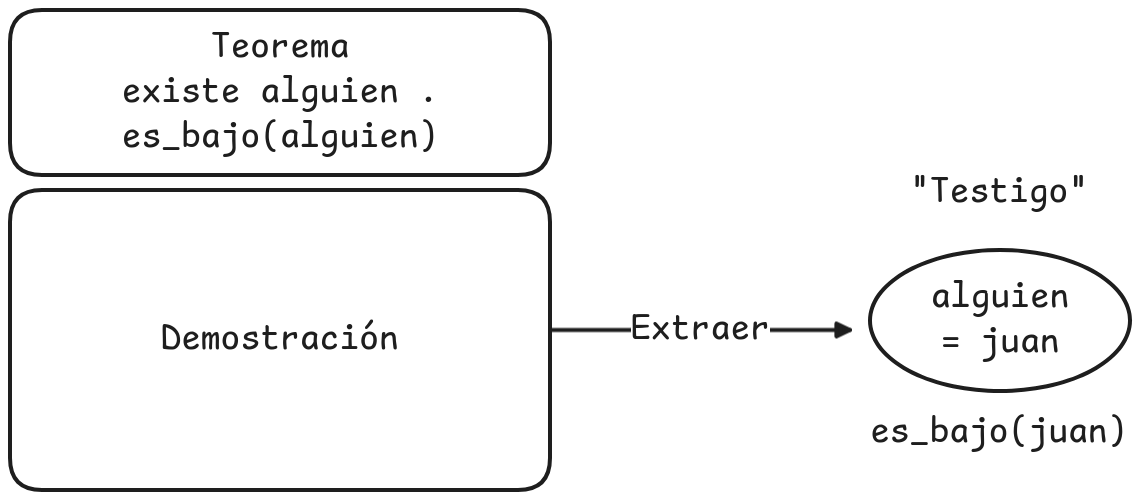
\includegraphics[scale=0.28]{img/ppt/extraction.png}
%     \end{figure}
% \end{frame}

\begin{frame}[fragile]{Extracción simple}
    \lstinputlisting[title=Extracción simple]{listings/ppt/extract/exists.ppa}

    \pause
    \begin{itemize}
        \item No es tan simple como buscar un \lstinline{take} (\ruleExistsI{}).
        \item \textbf{Útil}: Para demostraciones \textit{indirectas} o sin \lstinline{take} .
    \end{itemize}
\end{frame}


% \begin{frame}[fragile]{Extracción indirecta con instanciación}
%     \onslide<1->{\lstinputlisting[firstline=1,lastline=7]{listings/ppt/extract/parientes.ppa}}\vspace*{-\baselineskip}
%     \onslide<2->{\lstinputlisting[firstnumber=last,firstline=8,lastline=11]{listings/ppt/extract/parientes.ppa}}\vspace*{-\baselineskip}
%     \onslide<3->{\lstinputlisting[firstnumber=last,firstline=12]{listings/ppt/extract/parientes.ppa}}\vspace*{-\baselineskip}
% \end{frame}

% \begin{frame}[fragile]{Extracción indirecta}
%     Para extraer de
%     \begin{figure}
%         \centering
%         \lstinline{theorem todos_tienen_abuelo: forall A. exists B. es_abuelo(A, B)}
%     \end{figure}

%     Usando \ppaTool{},
%     \begin{figure}
%         \centering
%     \begin{minted}{shell-session}
% $ ppa extract parientes.ppa \
%     --theorem todos_tienen_abuelo \
%     --terms pepe
% Running program... OK! (size = 146)
% Translating... OK! (raw size = 136, reduced size = 9)
% Checking translated... OK!
% Extracted witness: padre(padre(pepe))
%        of formula: es_abuelo(pepe, padre(padre(pepe)))
% \end{minted}
% \end{figure}
% \end{frame}

% \begin{frame}
%     \lstinline{theorem todo_numero_tiene_leq: forall N. exists M . M <= N}

%     Extraemos un testigo \lstinline{cero} y podemos instanciar \lstinline{N} en lo que sea, por ej. \lstinline{cero <= 60}
% \end{frame}

% \begin{frame}{Extracción indirecta}
%     \lstinputlisting[title=Extracción indirecta]{listings/ppt/extract/indirect.ppa}
%     Extracción \textbf{indirecta} de \lstinline{theorem t2} nos da el testigo \lstinline{juan}.
% \end{frame}

% \begin{frame}{Extracción por el absurdo}
%     \lstinputlisting[
%         title=Extracción por el absurdo,
%         firstline=1,
%         lastline=9,
%     ]{listings/ppt/abs-ppt-narrow.ppa}
%     \pause
%     \begin{itemize}
%         \item En general $\fNot \forall \var .\fNot \anyForm \equiv \exists \var . \anyForm$.
%         \item Sin \lstinline{take} (\ruleExistsI) explícito, igual podemos extraer el testigo a partir del \lstinline{theorem} \lstinline{hayAlguienBajo}: \lstinline{juan}.
%         \pause
%         \item \alert{La implementación no es tan directa como buscar un \ruleExistsI} en el árbol de la demostración.
%     \end{itemize}
    
% \end{frame}

\begin{frame}{Lógica clásica}
    \begin{columns}
        \begin{column}{0.5\textwidth}
            \begin{itemize}[<+->]
                \item Buscamos un mecanismo general para extraer testigos de los certificados.
                \item Pero la lógica clásica \textbf{no es constructiva}, por LEM:
                \vspace{0.5cm}
                \proofTreeLEM
            \end{itemize}        
        \end{column}
        \begin{column}{0.5\textwidth}
            \begin{figure}
                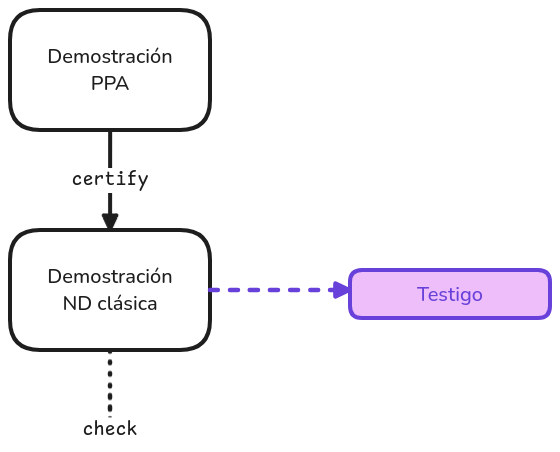
\includegraphics[scale=0.25]{img/ppt/extraction-candidate.png}
            \end{figure}
        \end{column}
    \end{columns}
%     \begin{block}{Mecanismo de extracción de testigos}
%         A partir de una demostración en PPA para una fórmula de la forma \[\forall \var_0 \dots \forall \var_n
% \exists \varTwo . \anyForm(\var_0, \dots, \var_n, \varTwo),\]

% \begin{enumerate}
%     \item la certifique generando una demostración en \alert<2>{deducción natural \textbf{clásica}}
%     \item  a partir de ella extraiga $\termTwo$ tal que, para $\term_0, \dots, \term_n$ cuales quiera, valga \[\anyForm(\term_0, \dots, \term_n, \termTwo)\]
% \end{enumerate}
%     \end{block}
\end{frame}

% \begin{frame}{Demostración no constructiva}
%     \begin{theorem}
%         Existen dos números irracionales $a$ y $b$ tales que $a^b$ es racional.
%     \end{theorem}
%     \begin{proof}
%         Considerar el número $\sqrt{2}^{\sqrt{2}}$. Por LEM, es o bien racional o
%     irracional.
%     \begin{itemize}
%         \item Supongamos que es racional. Como sabemos que $\sqrt{2}$ es
%               irracional, podemos tomar $a=b=\sqrt{2}$ que por hipótesis es racional.
%         \item Supongamos que es irracional. Tomamos $a = \sqrt{2}^{\sqrt{2}}, b
%                   = \sqrt{2}$. Ambos son irracionales, y tenemos

%               \[
%                   a^b
%                   = \left( \sqrt{2}^{\sqrt{2}} \right)^{\sqrt{2}}
%                   = \sqrt{2}^{\sqrt{2} \cdot \sqrt{2}}
%                   = \sqrt{2}^{2}
%                   = 2,
%               \]

%               que es racional.
%     \end{itemize}

%     En ambos casos podemos encontrar $a, b$ tales que $a^b$ es racional.
%     \end{proof}
    % \begin{itemize}
    %     \item ¡No nos dice quienes son $a$ y $b$! Complica la extracción de testigos.
    %     \item Pero podría: $a = \sqrt{2}$ y $b = 2 \log_2{3}$. \alert{No siempre}.
    % \end{itemize}
% \end{frame}

\begin{frame}{Demostración no constructiva}
    \begin{ejemplo}[Fórmula sin demostración constructiva]
        Sea $C$ algo indecidible (tipo \texttt{HALT}), queremos ver que vale
        \[
            \exists y .
                (y = 1 \fAnd \alert{C})
                \fOr
                (y = 0 \fAnd \alert{\fNot C}).
        \]
        \pause
        Podemos demostrarlo razonando por casos con LEM de $C \fOr \fNot C$

        \begin{itemize}
            \item Supongamos que vale $C$. Tomo $y = 1$.
            \item Supongamos que vale $\fNot C$. Tomo $y = 0$. \qed
        \end{itemize}
        
        \pause
        ¡No nos dice explícitamente si $y = 1$ o $y = 0$! No es \textit{constructiva}.
    \end{ejemplo}
    \pause
    ¿Entonces por qué lógica clásica?
    \begin{itemize}
        \item Permite razonar por el absurdo, con \ruleDnegE{} $\equiv$ \ruleLEM{}.
        \item Existen fórmulas que admiten \textit{solo demostraciones clásicas.}
        Ejemplo: \[\fNot (\form \fAnd \formTwo) \fImp \fNot \form \fOr \formTwo.\]
    \end{itemize}

    % \begin{theorem}[Teorema constructivo y no constructivo]
    %     Existen dos números irracionales $a$ y $b$ tales que $a^b$ es racional.
    % \end{theorem}
\end{frame}


\begin{frame}{Lógica intuicionista}
    \begin{center}
        \textbf{lógica intuicionista} = lógica clásica $-$ \ruleLEM{}
    \end{center}

    Características:
    \pause
    \begin{itemize}
        \item No tiene LEM\footnote{Ni principios de razonamiento equivalentes, como \ruleDnegE{}}, entonces siempre es constructiva.
        \pause
        \item Proceso de normalización con \textit{forma normal} buena, una demostración de un $\exists$ comienza con \ruleExistsI{}
        \proofTreeExistsI{}
        \item Siempre permite extracción de testigos.
    \end{itemize}
\end{frame}


% \begin{frame}{Clases de estrategias de extracción}
%     \begin{figure}
%         \centering
%         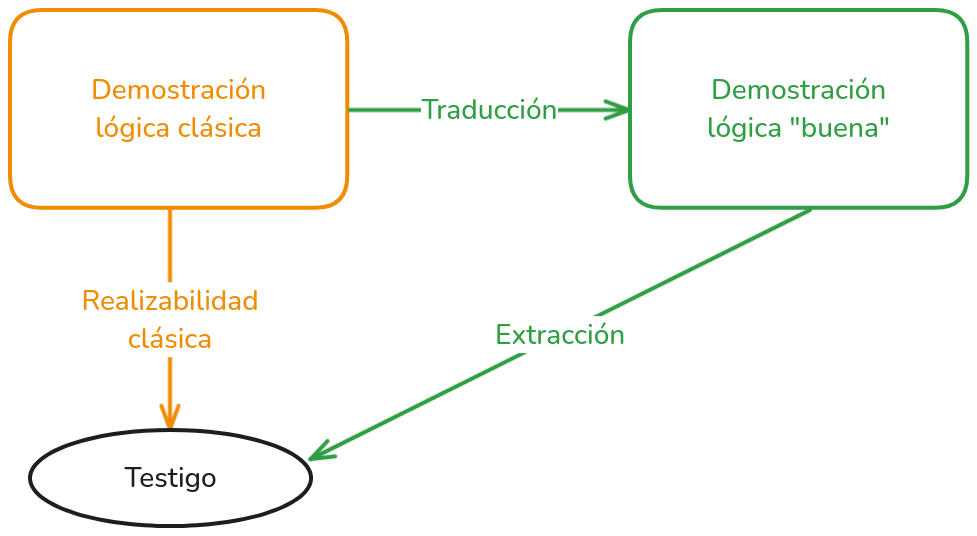
\includegraphics[scale=0.25]{img/ppt/extract-strategies.png}
%     \end{figure}
%     Clases de estrategias de extracción de demostraciones en lógica clásica:
%     \begin{itemize}
%         \item \textbf{Directas}: Extraer directamente de demostraciones clásicas. Técnicas de \textit{realizabilidad clásica} (Semánticas de $\lambda$-cálculos clásicos).
%         \item \textbf{Indirectas}: Convertir la demostración a una lógica que se porte mejor y extraer de ahí.
%     \end{itemize}
% \end{frame}


\begin{frame}{Estrategia de extracción indirecta}
    \begin{figure}
        \centering
        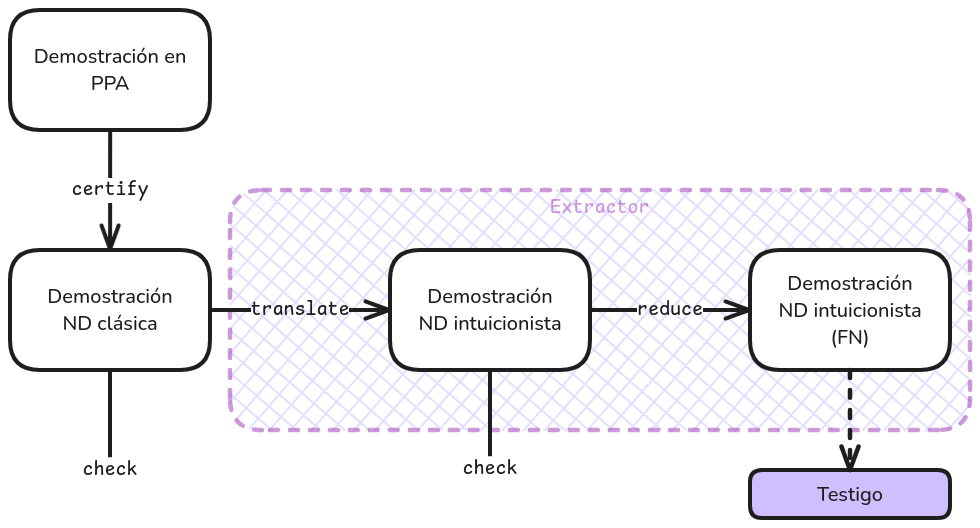
\includegraphics[scale=0.33]{img/arch.png}
    \end{figure}
\end{frame}

\subsection{Traducción de Friedman}

\begin{frame}{Traducción de doble negación}
    \begin{itemize}
        \item Queremos \textit{embeber} lógica clásica a intuicionista (no son equivalentes)
        \item Traducción de \textbf{doble negación}: método general.
        \item \textbf{Intuición}: ``agregar una doble negación a todo''.
        \item En clásica son equivalentes (\ruleDnegE{} $\equiv$ \ruleLEM{}) pero en intuicionista es más débil.
    \end{itemize}
    \pause
    \vspace{0.2cm}
    \begin{theorem}
        \begin{Large}
            \[
            \def\extraVskip{0.15cm}
            \AxiomC{$\someProof$}
            \noLine
            \UnaryInfC{$\ctx \bm{\judgC} \form$}
            \DisplayProof
            %
            \quad \rightsquigarrow \quad
            %
            \AxiomC{$\gN{\someProof}$}
            \noLine
            \UnaryInfC{$\gN{\ctx} \bm{\judgI} \alert<3>{\gN{\form}}$}
            \DisplayProof
        \]
        \end{Large}    
    \end{theorem}

    \pause

    \begin{alertblock}{Problema: Necesitamos la misma fórmula}
        \[
            \gN{(\exists \var . \form)} = \fNot \forall \var . \fNot \fNot \fNot \form
        \]
    \end{alertblock}
\end{frame}

\begin{frame}{El truco de Friedman}
    \begin{theorem}[Traducción de Friedman]
        Si tenemos
        \[ 
            \someProof \proves \ctx \alert{\judgC}
            \anyFormTwo
        \]

        Podemos generar una nueva demostración $\someProofTwo$ tal que
        \[ 
            \someProofTwo \proves \ctx \alert{\judgI}
            \anyFormTwo
        \]

        Si $\anyFormTwo$ y $\ctx$ cumplen con ciertas restricciones.
    \end{theorem}
\end{frame}

\begin{frame}{Traducción de doble negación relativizada}
    \begin{definition}[Negación relativizada]
        Podemos ver a $\fNot \form \equiv \form \fImp \fFalse$. Definimos
        \(
            \fNotR \form \equiv \form \rightarrow R
        \)
    \end{definition}
    \pause
    \begin{definition}[Traducción de doble negación relativizada]
            \vspace{-\baselineskip}
            \begin{align*}
                \transDNeg{\bot}                         & = R                                                             \\
                \transDNeg{\form}                        & = \fNotR\fNotR \form
                \quad \text{con $\form$ atómica}                                                                              \\
                \transDNeg{(\fNot \form)}                & = \fNotR \transDNeg{\form}                                          \\
                \transDNeg{(\form \fAnd \formTwo)}       & = \transDNeg{\form} \fAnd \transDNeg{\formTwo}                     \\
                \transDNeg{(\form \fOr \formTwo)}        & = \fNotR(\fNotR\transDNeg{\form} \fAnd \fNotR\transDNeg{\formTwo}) \\
                \transDNeg{(\form \rightarrow \formTwo)} & = \transDNeg{\form} \rightarrow \transDNeg{\formTwo}               \\
                \transDNeg{(\forall x . \form)}          & = \forall x . \transDNeg{\form}                                    \\
                \transDNeg{(\exists x . \form)}          & = \fNotR \forall x . \fNotR \transDNeg{\form}
            \end{align*}
    \end{definition}
\end{frame}

\begin{frame}{Funcionamiento de traducción de Friedman}
    Partiendo de
    \[
        \someProof \proves \ctx \judgC \anyFormTwo
    \]
    Queremos demostrar la misma fórmula en ND intuicionista. Pasos:
    \pause
    \begin{enumerate}[<+->]
        \item Aplicar traducción de doble negación relativizada (recursivamente a fórmula y demostración) tomando ``$R = \anyFormTwo$''.
        \[
            \tdn{\someProof} \proves \tdn{\ctx} \judgI \alert{\tdn{\anyFormTwo}}.
        \]
        \item Usarla para demostrar la fórmula original.
        
        \textbf{Restricción}: $\anyFormTwo$ debe ser $\classPiTwo$ con $\anyForm$ \textbf{conjuntiva}.
        \[
            \someProofTwo \proves \alert{\tdn{\ctx}} \judgI
            \forall \varTwo_1 \dots \forall \varTwo_n .
            \exists \var .
            \anyForm(\var, \varTwo_1, \dots, \varTwo_n).
        \]
        \item Mantener el contexto (reemplazando \ruleAx{} por $\form \judgI \tdn{\form}$)
        
        \textbf{Restricción}: Axiomas ($\ctx$) deben ser \textbf{F-fórmulas}.
        \[
            \someProofTwo' \proves \ctx \judgI
            \forall \varTwo_1 \dots \forall \varTwo_n .
            \exists \var .
            \anyForm(\var, \varTwo_1, \dots, \varTwo_n).\qed
        \]
    \end{enumerate}
\end{frame}

\begin{frame}{Tipos de fórmulas}
    \begin{definition}[Gramática de fórmulas]
        \begin{align*}
            \text{(atómicas)}\quad \form ::=\ & \fFalse \mid \fTrue \mid \pred(\term_1, \dots, \term_n)\\
            \text{(F-fórmulas)} \quad\fForm ::=\  &\form \\
            & \mid \fForm \fAnd \fForm \mid \fForm \fOr \fForm                       \\
            & \mid \forall \var . \fForm \mid \exists \var . \fForm                      \\
            & \mid \cForm \fImp \fForm                                                     \mid \fNot \cForm\\
            \text{(conjuntivas)}\quad \cForm ::=\ & A  \mid \cForm \fAnd \cForm
        \end{align*}
    \end{definition}
    \begin{lemma}
        Sea $\fForm$ una F-fórmula. Vale
        \(
            \fForm \judgI \tdn{\fForm}.
        \)
    \end{lemma}
    \begin{lemma}
        Sea $\cForm$ una fórmula conjuntiva. Vale
        \(
            \fNotR \cForm \judgI \fNotR \tdn{\cForm}.
        \)
    \end{lemma}
\end{frame}


\subsection{Normalización}

\begin{frame}{Normalización o reducción}
    \begin{center}
        \textbf{Motivación}: evitar \textit{``desvíos superfluos''}.
    \end{center}

    \begin{example}
        \[\ctxColor = \{\hypId_1: \form, \hypId_2: \formTwo \}\]
        Luego
        \[
    \AxiomC{}
    \RL{\ruleAxh{\hypId_1}}
    \UnaryInfC{$\ctxColor \judG \form$}
    \AxiomC{}
    \RL{\ruleAxh{\hypId_2}}
    \UnaryInfC{$\ctxColor \judG \formTwo$}
    \RL{\alert<2->{\ruleAndI}}
    \BinaryInfC{$\ctxColor \judG \form \fAnd \formTwo$}
    \RL{\alert<2->{\ruleAndEOne{}}}
    \UnaryInfC{$\ctxColor \judG \form$}
\DisplayProof
\pause
\quad
\rewrite
\quad
    \AxiomC{}
    \RL{\ruleAxh{\hypId_1}}
    \UnaryInfC{$\ctxColor \judG \form$}
    \DisplayProof
\]
    \end{example}
    \pause
    \begin{definition}[Reducción de conjunción]
        \[
            \reductionAnd
        \]
    \end{definition}
\end{frame}

% \begin{frame}{Curry Howard}
    

%     \begin{example}
%         Conjunciones como el tipo de las tuplas, y las eliminaciones como proyecciones.
%         \begin{align*}
%             \projectOne{\tuple{\lTerm_1}{\lTerm_2}} &\rewrite \lTerm_1\\
%             \projectTwo{\tuple{\lTerm_1}{\lTerm_2}} &\rewrite \lTerm_2
%         \end{align*}
        
%     \end{example}
% \end{frame}

% \begin{frame}{Normalización de implicación}
%     \begin{definition}[Normalización de implicación]        
%     \[
%         \AxiomC{$\someProof_\formTwo$}
%     \noLine
%     \UnaryInfC{$\ctx, \hypId: \form \judG \formTwo$}
%     \RL{\ruleImpIh{\hypId}}
%     \UnaryInfC{$\ctx \judG \form \fImp \formTwo$}
%     \AxiomC{$\someProof_\form$}
%     \noLine
%     \UnaryInfC{$\ctx \judG \form$}
%     \RL{\ruleImpE}
%     \BinaryInfC{$\ctx \judG \formTwo$}
%     \DisplayProof
%     %
%     \quad \rewrite \quad
%     %
%     \AxiomC{$\someProof_\formTwo\only<2->{\alert{\subst{\hypId}{\someProof_\form}}}$}
%     \noLine
%     \UnaryInfC{$\ctx \judG \formTwo$}
%     \DisplayProof
%     \]

%     \begin{itemize}
%         \item Primer idea: \xxcancel<2->{$\someProof_\formTwo \proves \ctx \judG \formTwo$} \pause
%         \item $\someProof_\formTwo$ requiere $\hypId : \form$, agregada por \ruleImpIh{\hypId}
%         \item Correcto: usar $\someProof_\formTwo$, pero \textit{sustituyendo} todas las ocurrencias de la hipótesis $\hypId$ por la demostración $\someProof_\form$ (sin capturas).
%     \end{itemize}
% \end{definition}
%\end{frame}
\begin{frame}{Algoritmo de reducción}
    \begin{definition}[Otras reglas]
        Además, hay reglas para simplificar
        \begin{itemize}
            \item \ruleExistsE{} con \ruleExistsI{}, \ruleForallE{} con \ruleForallI{}.
            \item \ruleNotE{} con \ruleNotI{}, \ruleOrE{} con \ruleOrI{}.
            \item \ruleImpE{} con \ruleImpI{}.
        \end{itemize}
    \end{definition}
    \begin{block}{Idea del algoritmo}
        Aplicar las reglas de reducción sucesivamente hasta que no se pueda y la demostración esté en \textit{forma normal}.
    \end{block}
\end{frame}

%\begin{frame}{Algoritmo de reducción}
%\textbf{Idea original}: reducir en un paso sucesivamente hasta que sea irreducible.
% \[
%     \def\defaultHypSeparation{\hskip .05in}
%     \AxiomC{$\someProof_\form$}
%     \AxiomC{$\someProof_\formTwo$}
%     \noLine
%     \BinaryInfC{$\vdots$}
%     \noLine
%     \UnaryInfC{$\someProof$}
%     \DisplayProof
%     \onslide<2->{
%     %
%     \underset{\left(\someProof_\form \rewrite \someProof_\form^1\right)}{\rewrite}
%     %
%     \AxiomC{\alert{$\someProof_\form^1$}}
%     \AxiomC{$\someProof_\formTwo$}
%     \noLine
%     \BinaryInfC{$\vdots$}
%     \noLine
%     \UnaryInfC{$\someProof$}
%     \DisplayProof
%     }
%     \onslide<3->{
%     %
%     \quad
%     \dots
%     \quad
%     %
%     \AxiomC{\alert{$\someProof_\form^*$}}
%     \AxiomC{$\someProof_\formTwo$}
%     \noLine
%     \BinaryInfC{$\vdots$}
%     \noLine
%     \UnaryInfC{$\someProof$}
%     \DisplayProof
%     }
%     \onslide<4->{
%     %
%     \underset{\left(\someProof_\formTwo \rewrite \someProof_\formTwo^1\right)}{\rewrite}
%     %
%     \AxiomC{$\someProof_\form^*$}
%     \AxiomC{\alert{$\someProof_\formTwo^1$}}
%     \noLine
%     \BinaryInfC{$\vdots$}
%     \noLine
%     \UnaryInfC{$\someProof$}
%     \DisplayProof
%     %
%     \dots
%     }
% % \]

% \begin{itemize}
%     \item \textbf{Algoritmo}: Reducir sucesivamente hasta que sea irreducible.
%     \item \textbf{Estrategias de reducción}: en un paso o muchos pasos.
%     \item \textit{Gross-Knuth}: reduce en muchos pasos todos los sub-términos posibles al mismo tiempo.
% \end{itemize}


% En un solo paso,
% \[
%     \AxiomC{$\someProof_\form$}
%     \AxiomC{$\someProof_\formTwo$}
%     \noLine
%     \BinaryInfC{$\vdots$}
%     \noLine
%     \UnaryInfC{$\someProof$}
%     \DisplayProof
%     %
%     \pause
%     \underset{
%         \left(\begin{aligned}
%             \someProof_\form &\overset{*}{\rewrite} \someProof_\form^*\\
%             \someProof_\formTwo &\overset{*}{\rewrite} \someProof_\formTwo^*
%         \end{aligned}
%         \right)
%     }{\rewrite}
%     %
%     \AxiomC{\alert{$\someProof_\form^*$}}
%     \AxiomC{\alert{$\someProof_\formTwo^*$}}
%     \noLine
%     \BinaryInfC{$\vdots$}
%     \noLine
%     \UnaryInfC{$\someProof$}
%     \DisplayProof
%     \]
% \end{frame}

% \begin{frame}{Programa con falla de extracción}
%     \begin{columns}
%         \begin{column}{0.5\textwidth}
%             \lstinputlisting{listings/ppt/extract/or-fail.ppa}
%         \end{column}
%         \begin{column}{0.5\textwidth}
%             Certifica el programa generando una demostración que en lugar de comenzar con \ruleExistsI{}, comienza con \ruleOrE{} y en cada rama introduce el existencial dos veces, con el mismo término
%         \end{column}
        
%     \end{columns}
% \end{frame}

\section{Detalles de implementación}

\begin{frame}{Parser y lexer}
    \begin{figure}
        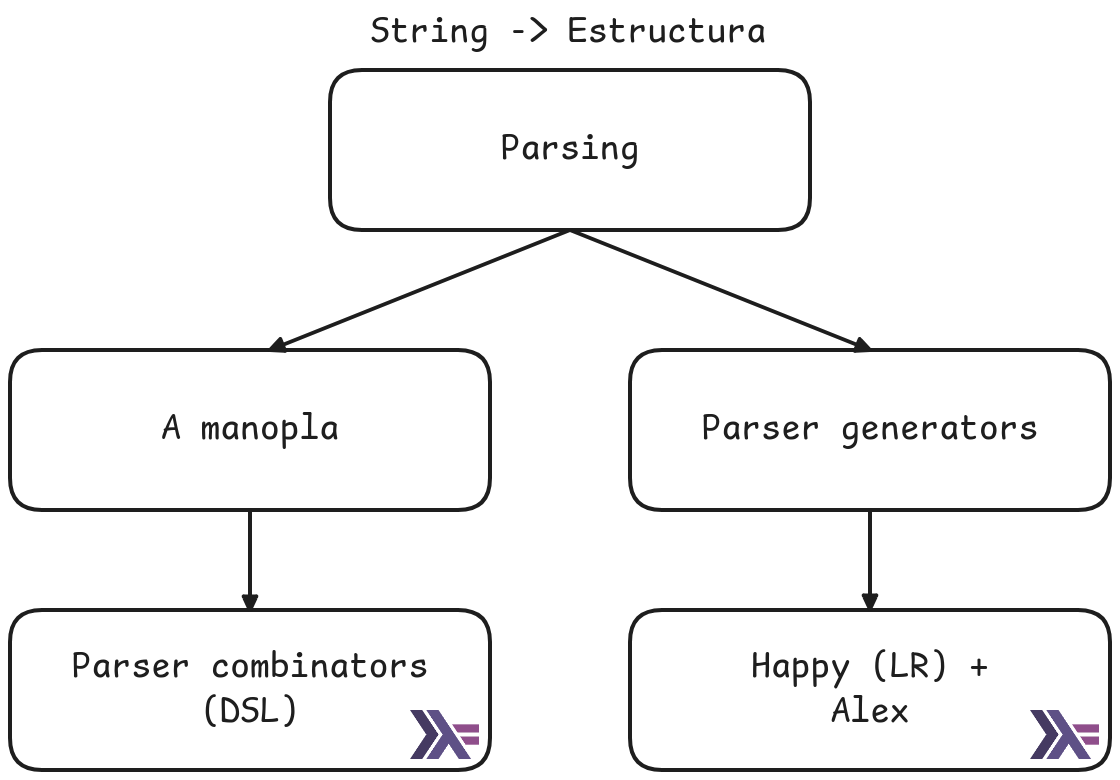
\includegraphics[scale=0.28]{img/ppt/parsers.png}
    \end{figure}
\end{frame}

\begin{frame}{La herramienta \ppaTool{}}
    \begin{figure}
        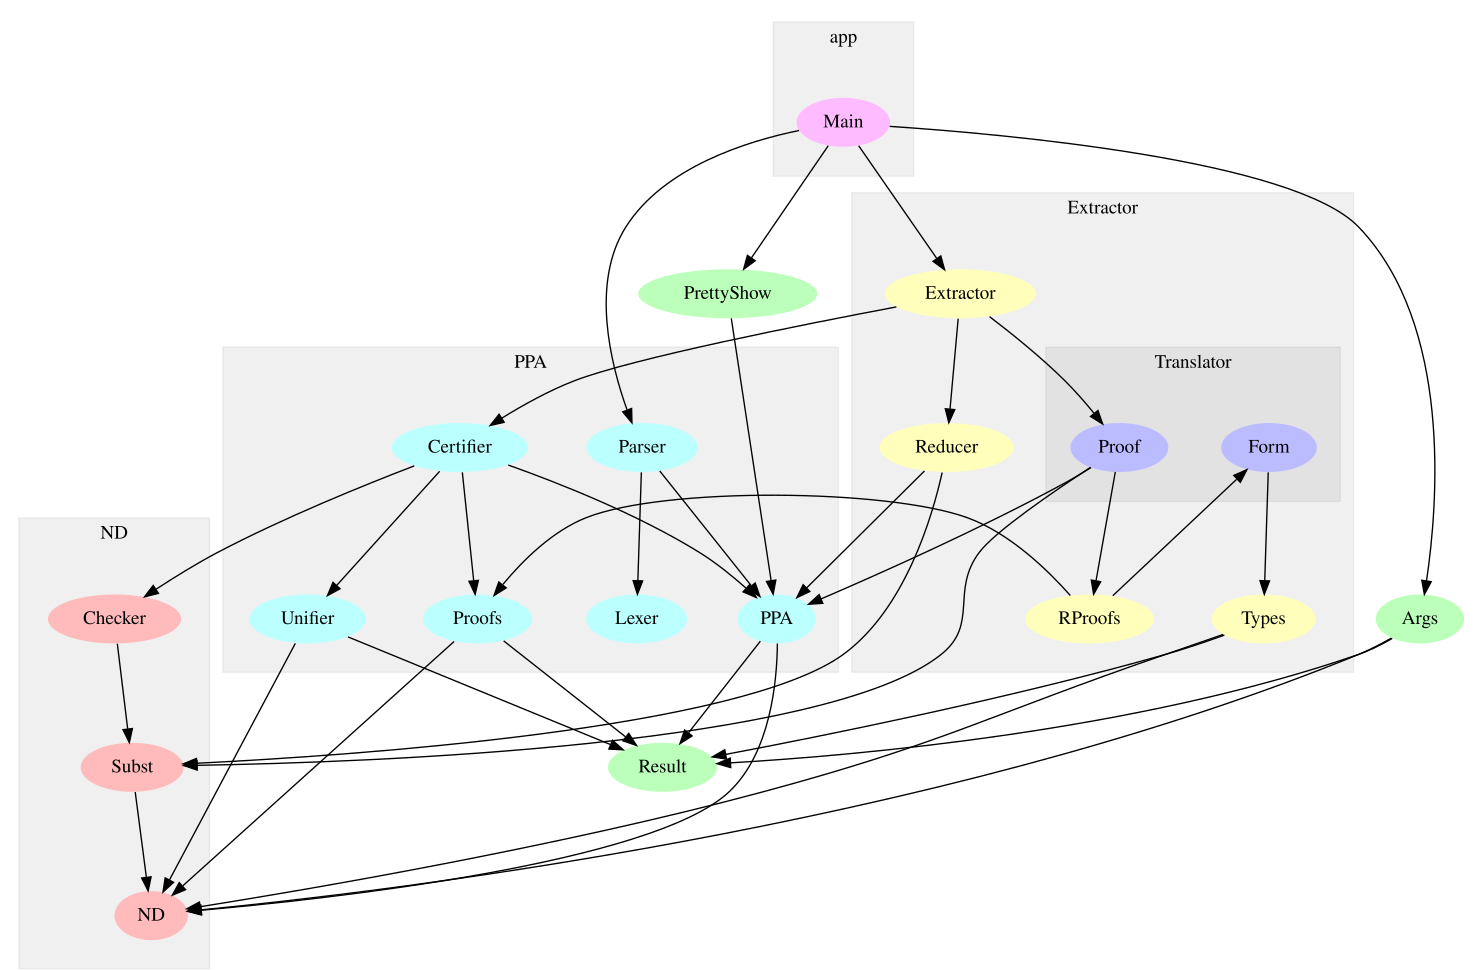
\includegraphics[scale=0.285]{img/modules.png}
        \centering
        \small Haskell, 19 módulos con 330 tests
    \end{figure}
    % Aprovechar para hacer un repaso
\end{frame}



\section{Conclusiones}

\begin{frame}{Conclusiones - PPA}
    \begin{itemize}[<+->]
        \item Diseñamos e implementamos \ppaTool{}: un asistente de demostración, junto con el lenguaje \ppaLang{}.
        \item Los programas se \textbf{certifican} generando demostraciones en \textit{deducción natural}.
        \item Mecanismo heurístico de demostración automática: \lstinline{by}. 
        
        \textbf{Extensión}: Hacerlo recursivo permitiendo eliminar los universales de más de una hipótesis.
        \item Desafíos
        \begin{itemize}
            \item Haskell.
            \item Demostraciones generadas automáticamente difíciles de \textit{debuggear}.
        \end{itemize}
        \item Otras mejoras
        \begin{itemize}
            \item Permitir importar archivos, implementar biblioteca estándar.
            \item Extender PPA con tipos (usando LPO \textit{many-sorted} con géneros).
            \item Modelar de forma nativa inducción (segundo orden) e igualdad.
            \item Mejorar reporte de errores (\textbf{muy} bajo nivel).
        \end{itemize}
    \end{itemize}
\end{frame}

\begin{frame}{Conclusiones - Extracción de testigos}
    Implementamos un mecanismo de \textbf{extracción de testigos}: composición de traducción de Friedman y reducción de ND intuicionista.

    \begin{itemize}[<+->]
        \item \textbf{Desafío}: Problemas aparecieron en la integración de las 3 partes.
        \item Traducción de Friedman
        \begin{itemize}
            \item \textbf{Extensión}: A más de un $\exists$.
            \item \textbf{Desafío}: Demostraciones de F-fórmulas y conjuntivas.
            \item \textbf{Limitación}: Refinar la definición de fórmulas conjuntivas y explorar aparente vínculo con \textit{fórmulas de Harrop}.
        \end{itemize}

        \item Reducción
        \begin{itemize}
            \item Solo contempla introducciones y eliminaciones del mismo conectivo.
            \item \textbf{Incompleta}: no contempla \textit{reducciones permutativas}. \textit{Mejora}: Implementarlas. Ejemplo que queda afuera: \lstinline{cases} (\ruleOrE{}).
            \item \textbf{Ineficiente}: en cada paso reinicia la búsqueda de todos los focos de evaluación. \textit{Mejora}: Usar una \textit{máquina abstracta}.
        \end{itemize}
    \end{itemize}
\end{frame}

\begin{frame}{Fin}
    \begin{Huge}
        \begin{center}
            ¡Gracias!
        \end{center}
    \end{Huge}
    \begin{figure}
        \centering
        
\includegraphics[scale=0.35]{img/ppt/qr-ppa.png}
        \caption*{github.com/mnPanic/tesis}
    \end{figure}
\end{frame}

\end{document}